\section{Multichannel RPL Protocol}

%ContikiMAC \cite{contikimac} is the default low power listening MAC protocol in Contiki. It was proved to be efficient in a single channel \cite{micmac}\cite{orpl}. ContikiMAC uses periodical wakeups to listen to the neighbours transmission packet. It has a phase-lock mechanism to learn the neighbours wake-up phase to enable efficient transmissions and a fast sleep optimisation in case of spurious radio interference is detected.

%routing in RPL
%Routing protocol for low power and lossy networks (RPL) is a gradient based routing protocol forming any-to-any routing for low power IPv6 networks. RPL topology is a Destination-Oriented Directed Acyclic Graph (DODAG), rooted at LPBR with no cycles. The root has the overall view of the network. The other nodes however, only has knowledge of its neighbours and default router. RPL is a rooted topology which any-to-any traffic is directed towards the root unless the common ancestor is found which the traffic is then routed downwards towards the destination. This strategy is used in order to scale large networks by reducing the routing overhead at the cost of increased hop count through common ancestor. %However, RPL has drawbacks. It takes a while before a broken link is detected and global repair to take place.

%objective function
%routing metrics
%In RPL terminology, the node distance to the root and other nodes is defined as the node's rank. RPL finds the path with the minimum number of transmissions that a node expect to successfully deliver a packet to the destination and switches only if it is less than the current rank to prevent frequent changes~\cite{mrhof}.

%RPL separates the routing optimisation objectives with the packet processing and forwarding policies. This allows the networks to have different optimisation objectives which include the rank computation, node selection, parents selection and route optimisation. However, RPL Objective Function (OF) is not an algorithm. It is the process to optimise the routes. In RPL terminology, the node distance to the root and other nodes is defined as the node's rank. The rank increases downwards and decreases towards the root. There are two Objective Functions specified as the standard, which are the Objective Function Zero (OF0) and Minimum Rank with Hysteresis Objective Function (MRHOF). OF0 is based on the shortest amount of hops to the root~\cite{of0}. MRHOF uses hysteresis with the Expected Transmission Count (ETX) metric. ETX is the number of transmissions that a node expect to successfully deliver a packet to the destination. It finds the path with the minimum rank and switches only if the rank is less than the current rank to prevent frequent changes~\cite{mrhof}. Hop count and ETX are node and link metrics which is a direct conversion of metric to rank values. By default, Contiki uses MRHOF.

%rpl messages
%RPL defines three main types of ICMPv6 based control messages used in topology formation and maintenance which are the DODAG Information Object (DIO), Destination Advertisement Object (DAO) and DODAG Information Solicitation (DIS). DIO contains the information needed by the node such as the configuration parameters, parent selection and rank. DAO is used to enable packets to propagate towards the root. DIS is used by a node to require  DIO messages from its neighbour in order to join the DODAG.

Multichannel RPL concentrates on finding the best channels for nodes to listen and transmit on, given policies that needs to be complied. 

\subsection{Overview}

%\explain the ideas (state machine?), reasons for doing

The design of Multichannel RPL are based on several crucial observations:

\begin{itemize}
\item Channel assignment - as the nodes are battery powered, the decision of selecting the channel is left to LPBR. This reduces the processing on the nodes and enable load balancing within channels as LPBR has a complete knowledge of the topology. LPBR keeps track of the channel conditions based on the feedback it receives from the nodes. All intelligence is done at LPBR.

\item Interference - external interference cannot be predicted, thus channel cannot be allocated beforehand as it varies over time. It is impossible to determine a single channel that is free from interference.

\item Frequency diversity - RPL only considers a single channel. Applying multichannel to the existing RPL may hinder neighbour detection and RPL control messages. We solved this by enabling unicast in neighbour detection and RPL control messages. We assume that no new nodes should join the topology after the initial setup.
\end{itemize}

Multichannel RPL focuses on the application layer of the protocol. The selection of channels to the nodes are decided once the topology tree has been formed by LPBR.

%Figure 1 shows the design of Multichannel RPL. The states are explained in the next sections.

%\begin{figure}
%\centering
%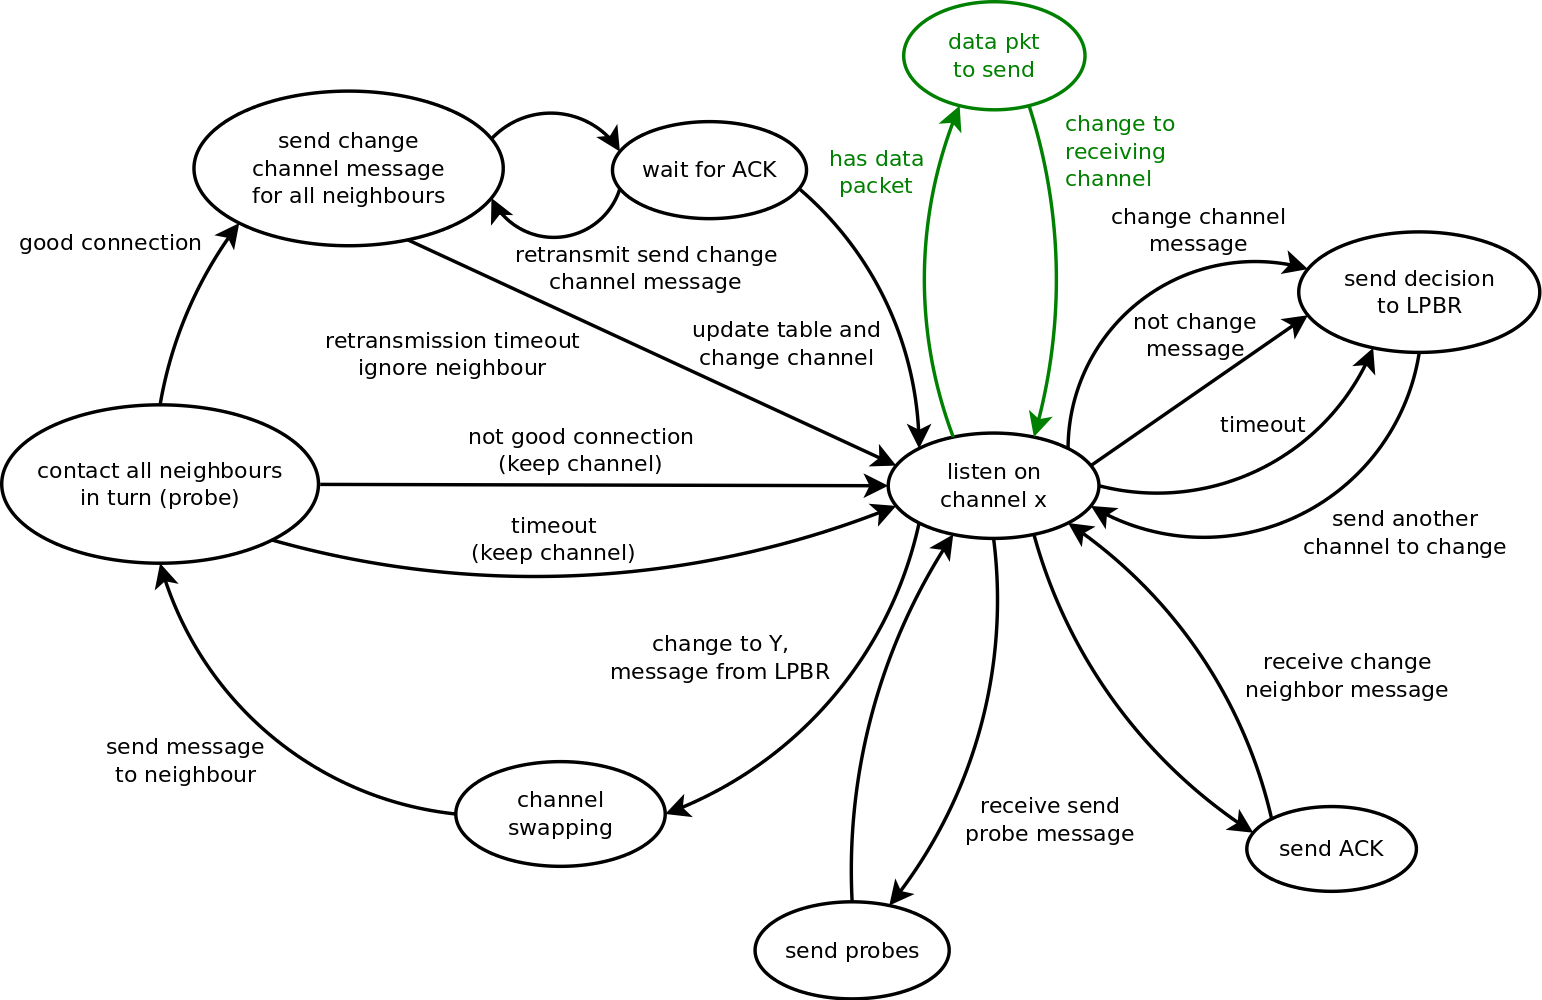
\includegraphics[height=7.2cm]{stateDiagram}
%\caption{State machine for channel switching.}
%\label{fig:example}
%\end{figure}

\subsection{Channel Selection Strategies}

%//LPBR decides the channel; random at first (or maybe not) and then based on probing that were done previously stating the condition of channels.

At initialisation, during the tree topology formation, all nodes are on the same channel, which is channel 26 by default. This is because nodes that are on different channels might not be detected which result in unoptimised topology. Channel 26 is used because it is the channel that the studies in \cite{chrysso}\cite{micmac}\cite{watteyne} have in common. By default, in a single channel case, channel 26 is used as it usually does not overlap with WiFi and is relatively in a cleaner frequency than the other channels. 

%Once the topology has formed and stabilised, LPBR sends a channel change message which random channel is chosen for the node to change into. LPBR chooses random channel as it does not have information regarding the condition of the channels. It will build it's knowledge of the channels based on the feedback it receives from the nodes. If LPBR has the knowledge of the channels, it decides on the best channel for the node to maintain high transmitting and receiving rate. LPBR set a timer for the node to reply. If it times out, no changes in done to the channel.

%The channel that is selected also needs to (fulfil?) two hops colouring strategies which is explained in detail in the next section. This is done in order to eliminate the risk of next hop neighbour using the same channel which could lead to congestion on the channel.

%how often probing? each time?

There are two strategies that LPBR uses when deciding on a channel change; random change and two hop colouring strategy. 

\subsubsection{Random Channel Selection -}
At initialisation, LPBR uses random channel to decide which node and what channel the node should try to change into. The neighbours of the node will send probes messages to check the channel condition and the probing result is used to decide on the changes. This strategy is used when LPBR has no knowledge of the suitable channel for the node. By forcing the neighbour-node pair sending probing messages, LPBR could build its knowledge based on the probing results. LPBR will have an overall information of channels which will affect its decision in the future. The advantages of having these information is that LPBR can be certain that the channel that it chooses for a node to change into will have better throughput than the current channel. Through probing results, LPBR knows how much better a certain channel is compared to other channels. This information is only accessible by the LPBR. 
	
%**TWO HOP COLOURING STRATEGY?
\subsubsection{Two Hops Neighbour Strategy -}
In two hops neighbour strategy, similar to random channel selection, LPBR chooses a random channel for a node unless LPBR has full knowledge of the channels condition as mentioned in Random Channel Selection section. LPBR keeps the information of each node neighbours and channel in a table. The random channel that was selected is checked with the information in the table. to decide if there is another node that is two hops away using the same channel. If the channel is being used, a new channel is selected and checked. The reason for this is to spread the workload on different channels so that more transmissions are able to take place at the same time. However, if a two hops free channel is not found, the default channel 26 is used. Once the new channel is selected, the channel quality is checked before it is used to replace the previous channel.

%In LPBR, before it sends a channel change message, LPBR will decide on a new channel. In the beginning, LPBR has no knowledge of channels that could give optimal transmission success rate. LPBR will choose a random channel value from channel 11 to 26. The default channel in a single channel network is channel 26. The chosen channel is checked if other node within two hops are using it. 

%In RPL, the node routing table and neighbour table do not contain the information of all existing nodes in the network but only the nearest nodes that are in range. The neighbour table keeps the information of the node's neighbours listening. This is important as the node should always sends on the correct transmitting channel which is the neighbour listening channel. 

%///WRONG! LPBR DO THE 2 HOPS CHECKING!!!
%When a node gets the channel to change into, it first checks it's own neighbour table if any of the neighbour is currently on the channel. If there is none, the node asks the neighbours to check their neighbour table. The decision of whether the channel can be used is passed back to LPBR. LPBR will then use the channel or decide on another channel depending on the reply from the node and neighbours, and the steps explained in section 3.4 proceed. 

%If LPBR could not get a two hops free channel, it will use the default channel which is channel 26.

\subsection{Channel Quality Checking}
%channel quality check = probing
%//Channel condition is checked by probing before deciding to switch unless LPBR has the information regarding the specific channel based on probing that were done previously.

The channel is checked at initialisation in order for the LPBR to build it's knowledge on the channels quality. The channel quality checking is invoke each time the node receives the channel change message from LPBR. The node informs all the neighbours in turn, of the new channel it will be listening on. The node's neighbours will probe the node and the node collects the information on the success or failure rate of the channel. The results from probing is used to decide if the new channel is better than the current channel. LPBR is informs and updates its knowledge on the channel condition.

***probing tries to avoid the interference channel.

The channel is not chosen either if it timed out or the probing messages received are below a threshold. The node will revert to the previous channel as it is better than the new channel selected. However, due to ContikiMAC nature of only able to end 8 packets per second, we did not run the probing long enough to be able to completely eliminate the interference channel. The interference channel might be used by some nodes if during the probing, all probing messages are received. We could increase the number of probing messages by increasing the buffer size or the radio duty cycle (to be confirmed!!) but we chosen not to because increasing buffer size means that we will be using more memory which is not practical as we have limited memory available. If we increase the radio duty cycle, that would cost us more energy as the node will be awake more frequent and the nodes will not be in sync as they would have different radio duty cycle. That would increase the chance of packet loss. Our other option is to run the probing for a longer time.

%////FUTURE WORK?
%Even though external interference varies over time, it is unlikely that the channel quality fluctuates frequently within minutes that would affect the receiving success rate. Thus, the channel quality check is invoke on three (cases? situations?); on initialisation, when receiving LPBR channel change message and when the packet delivery ratio (PDR) drops. ***NOT SURE  


%****
%Each node keeps the counter of packets it has sent and received. It will send the information to LPBR periodically in order for LPBR to get a full view on the condition of the channels. LPBR will then decide if the node needs to change to another channel depending on the sent and received information. If the node does not perform well based on the number of received packets less than the number of packets being sent, LPBR will decide on a new channel the node needs to change into. The node will go through the channel changing processes to decide if the new channel is performing better than the previous channel before (settling?) for the new channel.

\subsection{Channel Switching}

%//explain LPBR that decides whether the nodes should stay on the same channel or switch to a new channel based on the information it gathers through nodes probing.

%State machine explanation should be here?

\begin{figure}
\centering
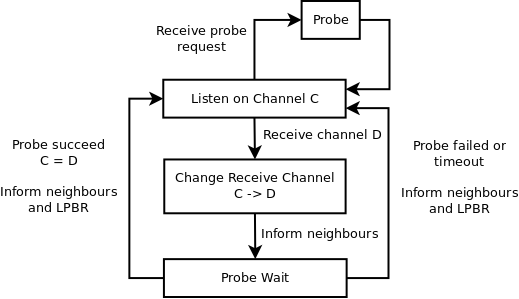
\includegraphics[width=3in]{Diagram1}
\caption{Channel switching process}
\label{fig_sim}
\end{figure}

LPBR decides the channel that a node should be listening on either by random selection or through LPBR knowledge of the channels. Figure 1 shows the states in channel switching. LPBR sends the change channel message to the node on the receiving node current listening channel. The node saves it's current and new channel to allow the channel to be restored if require. The node contacts its neighbours, informing the new channel value. The neighbours will in turn, send probing messages to check the new channel condition. Different neighbours might have different success rate, thus the final decision of switching is based on the threshold that is set. 

If the threshold is not met or the probing has timed out, the node is restores to its current channel and informs LPBR of the updated channel condition. Otherwise, the node sends a change channel message to the neighbours and waits for acknowledgement. The node and the neighbours updates their table. The node informs LPBR of the changes and listens on the new channel for data packets. If the acknowledgement does not arrive after the timeout, the change channel confirmation message is retransmitted. The neighbour node is ignored if the retransmissions has timed out. 

%It is possible that the node itself ask for a channel change if its PDR is below a threshold. LPBR checks and updates the information of the channels and sends a change channel message. The steps as previously explained are repeated. ***NOT SURE? LPBR asks for the transmission and receiver rate periodically from all the nodes to decide a channel change.

%LPBR sends a change channel message after ***some time to check the condition of the node's channel and to get updates on the channels. The node's neighbours will start probing on the channel which the result is use to decide the changes.

%\subsection{LPBR Strategies}   
